\chapter{Introduction}

This report aims at being a short documentation on the Microelectronic Systems course project at the first year of the master degree both in Computer and Electronics Engineering at Politecnico di Torino. \newline
The target is the \textbf{design} and the \textbf{implementation} phase of a pipelined processor by VHDL, as is described in \cite{book:rif.1}, followed by a simple \textbf{synthesis} and a \textbf{physical layout} definition. The main flow has passed through the following steps:
\begin{enumerate}
\item Design and implementation at RTL level
\item Simulation by assembly codes
\item Synthesis and gathering results about timing, area and power consuption
\item Realization of the physical layout
\end{enumerate}

For 1 and 2, I used the \textit{Xilinx ISE Design Suite 14.7}, although during the laboratory sessions the tool was \textit{ModelSim}. I made this choice because I think it's better both from the management of files point of view and for the more intuitive interface of the simulation tool. The synthesis step has been performed by \textit{Synopsys' DesignVision}, whose license has been granted to the Politecnico di Torino. In order to use it, I haved to use a virtual machine, running on \textit{Linux}, provided by the Department of Electronics and Telecommunications servers. Same conditions for the last step, by \textit{Cadence Innovus Implementation System}. Moreover, I liked exploiting \textit{GitHub} functionalities to make easier the passage of data from my \textit{Windows} laptop and the virtual machine; you can download it from \url{https://github.com/sandrosalvato94/MyDLX}

\section{Basic vs Pro version}

Specification are described in \cite{ProjectSpecification}, you can find it among files in Documents directory. Summarizing, basics features for the Basic version are:
\begin{itemize}
\item \textbf{Pipeline}
\item \textbf{Simple instruction set} (see below)
\item \textbf{Simple datapath}
\item \textbf{Basic synthesis}
\item \textbf{Basic physical design}
\item This \textbf{report}
\end{itemize}

\begin{figure}[H]
\centering
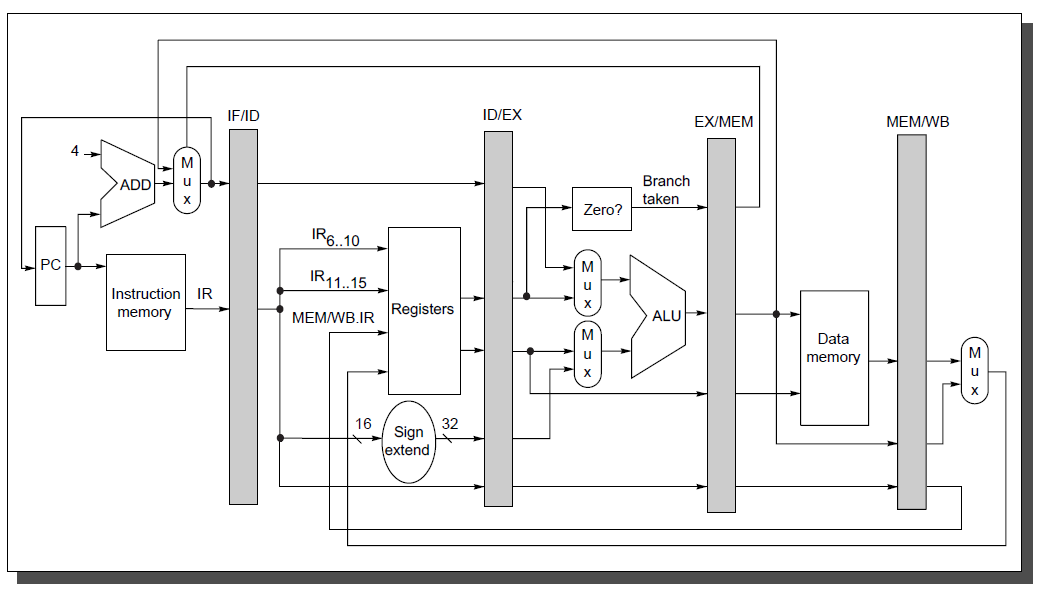
\includegraphics[scale=.7]{Immagini/00}
\label{00}
\caption{Basic DLX Datapath. \textit{Figure 3.4 from \cite{book:rif.1}}}
\end{figure}

Among pro hints, these are reported:
\begin{itemize}
\item \textbf{Extended instruction set} (see below)
\item \textbf{Extended datapath}
\item \textbf{Windowing}
\item \textbf{Control Hazard}
\item \textbf{Optimization of the power consuption}
\item \textbf{Caching}
\item \textbf{Advanced synthesis}
\item \textbf{Advanced physical design}
\item \textbf{Whatever I wanted...}
\end{itemize}

I targeted the pro version, exploring and implementing the following features:
\begin{itemize}
\item 
\end{itemize}